\documentclass[12pt, a4paper]{article}

\usepackage{graphicx}
\usepackage{amssymb}
\usepackage{amsmath}
\usepackage{hyperref}
\usepackage{physics}


\title{PSet7 Report}
\author{Ali Abolhassanzadeh Mahani}

\begin{document}
	\maketitle
	\section{Implementing Code to Simulate the Ising Model}
	I started this code by making the class \texttt{Ising} with an \texttt{\_\_init\_\_} function that 
	takes in the size of the platform, $L$, and $\beta$, and then creates a grid of size $L$ and fills it
	randomly with $\pm1$ as spin up/down. ($\ket{\uparrow}, \ket{\downarrow}$)\\
	
	We know that the distribution for this system is canonical, of the form
	$Z = \sum_{i}^{} e^{-\beta E_i}$. So now, I create a method \texttt{metropolis()}, which uses the metropolis algorithm to make the distribution of energy $E_i$ to be of the canonical form.
	This method, loops for $L^2$ times and picks a cell on the grid randomly and performs the metropolis conditions on it and if it's works, the method give the cell a bit flip.
	
	Here I initialized an Ising model of size $L = 1000$ and called the \texttt{metropolis()} 
	function on it 100 times. the results are available in Fig\ref{fig:ising_grid}
	\begin{figure}
		\centering
		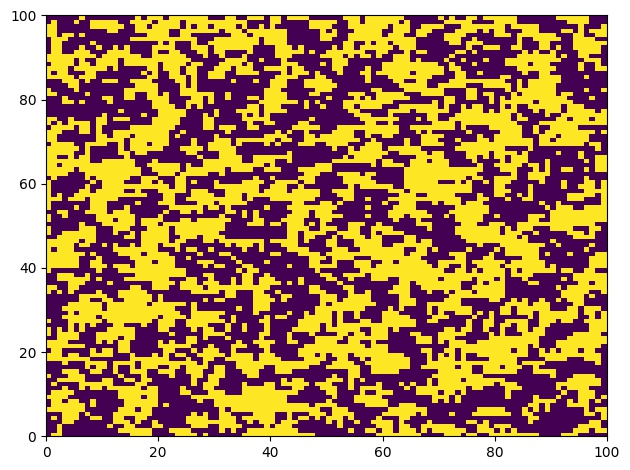
\includegraphics[width=0.8\linewidth]{../ising.jpg}
		\label{fig:ising_grid}
		\caption{Ising model of size 1000, before and after using the \texttt{metropolis()} function 100 times.}
	\end{figure}
	
\end{document}